
\subsection{Controller design}
 
\begin{figure}[h!]
    \begin{center}  
    \includegraphics[width=\columnwidth]{block-diagram.png}    
    \end{center}
    \caption{Block diagram}
    \label{fig:controller1}
\end{figure}

We found the most important part of our design to be having zero steady state error, being able to aim confidently down a certain sighting. So, we determined our controller would have an integrator term. We decided our system must have under 5\% peak overshoot, and must have rise time of under \SI{0.5}{\second}, to ensure the system can quickly aim down a bearing very close to the actual target.

A PID controller was decided upon, to get initial gain values, $\omega_n$ and $\zeta$ were solved for using our desired transient response. From here gains were adjusted and tested with the \lstinline{stepinfo} function until a desirable control response was reached. The control gains are as follows:
Positive Rotation: Kp=3 Ki=1   Kd=3
Negative Rotation: Kp=6 Ki=0.5 Kd=12.2
The response in both directions can be seen by the following simulations:

\begin{figure}[h!]
\centering
    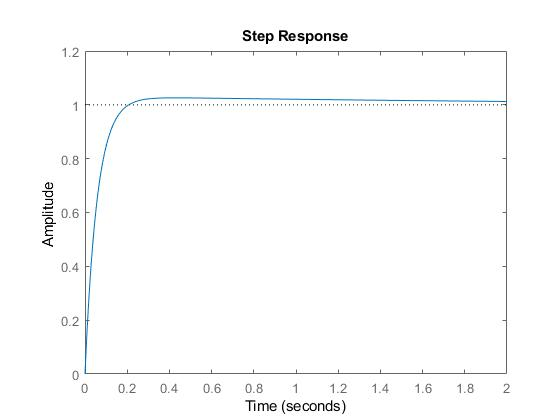
\includegraphics[scale=.4]{posPID.jpg}
    \caption{ Positive PID Transfer Function}
    \label{fig:pos responce}
\end{figure}
\begin{figure}[h!]
    \centering
    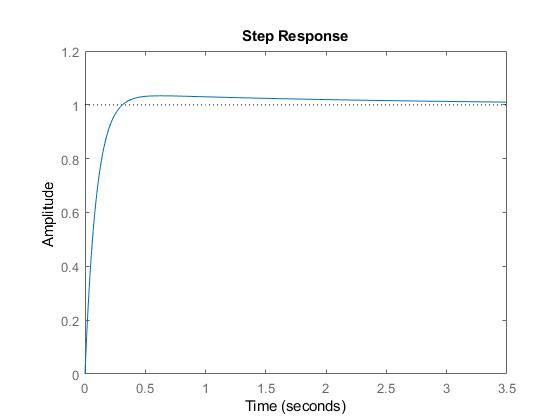
\includegraphics[scale=.4]{negPid.jpg}
    \caption{Negative PID Transfer Function}
    \label{fig:neg responce}
\end{figure}